%  LaTeX support: latex@mdpi.com
%  Revised MDPI Diagnostics manuscript (Track A: baseline artifacts + full methodological,
%  mathematical, analytical-complexity, and reporting revisions).
%  Toggle \rev macro below for clean vs. highlighted revision copy.

%====================================================
\documentclass[diagnostics,article,submit,moreauthors]{Definitions/mdpi}
%=====================================================
% MDPI internal commands - do not modify
\firstpage{1}
\makeatletter
\setcounter{page}{\@firstpage}
\makeatother
\pubvolume{1}
\issuenum{1}
\articlenumber{0}
\pubyear{2026}
\copyrightyear{2026}
\datereceived{5 November 2026}
\daterevised{ }
\dateaccepted{ }
\datepublished{ }

%=================================================================
\usepackage{graphicx}
\usepackage{amsmath,amssymb,amsfonts}
\usepackage{booktabs}
\usepackage{xcolor}
\usepackage{url}
\usepackage{tikz}
\usetikzlibrary{shapes.geometric, arrows.meta, positioning, calc}

% Revision highlight helper: clean copy renders normal text.
\newcommand{\rev}[1]{\textcolor{blue}{#1}}

%% --- Palette + styles for the system diagram (Fig. 1) ---
\definecolor{accent}{HTML}{0D9488}
\definecolor{accentlt}{HTML}{CCFBF1}
\definecolor{heavy}{HTML}{4338CA}
\definecolor{heavylt}{HTML}{E0E7FF}
\definecolor{alert}{HTML}{EA580C}
\definecolor{alertlt}{HTML}{FFEDD5}
\definecolor{muted}{HTML}{475569}
\definecolor{mutedlt}{HTML}{F1F5F9}
\tikzset{
  io/.style={rectangle, rounded corners=2pt, draw=muted, fill=mutedlt, thick, align=center, font=\scriptsize, inner sep=4pt, minimum height=0.8cm},
  light/.style={rectangle, rounded corners=3pt, draw=accent, fill=accentlt, very thick, align=center, font=\scriptsize, inner sep=4pt, minimum height=0.9cm},
  heavyblk/.style={rectangle, rounded corners=3pt, draw=heavy, fill=heavylt, very thick, align=center, font=\scriptsize, inner sep=5pt, minimum height=1cm},
  decision/.style={diamond, aspect=2.2, draw=alert, fill=alertlt, very thick, align=center, font=\scriptsize, inner sep=1pt},
  proc/.style={rectangle, rounded corners=3pt, draw=muted, fill=white, thick, align=center, font=\scriptsize, inner sep=4pt, minimum height=0.8cm},
  flow/.style={-{Stealth[length=2mm,width=1.5mm]}, thick},
  flowlab/.style={font=\scriptsize\itshape, fill=white, inner sep=1.5pt},
}

%=================================================================
\Title{TCR-P: A Tiered Confidence-Routing System for Pneumothorax Detection in Chest Radiographs}

\newcommand{\orcidauthorA}{0000-0002-0046-1064}
\newcommand{\orcidauthorC}{0000-0001-6800-9878}
\newcommand{\orcidauthorD}{0000-0001-6254-9291}

\Author{Daniela-Maria Cristea $^{1,2}$\textsuperscript{\textdagger}\orcidA{}, Alperen Y\"or\"uk $^{3}$\textsuperscript{,\textdagger}, Henning M\"uller $^{4}$\orcidC{} and L\'aszl\'o Barna Iantovics $^{5,}$*\orcidD{}}

\AuthorNames{Daniela-Maria Cristea, Alperen Y\"or\"uk, Henning M\"uller and L\'aszl\'o Barna Iantovics}

\address{%
$^{1}$ \quad Department of Computer Science and Engineering, ``1 Decembrie 1918'' University of Alba Iulia, Alba Iulia, Romania; daniela.cristea@uab.ro\\
$^{2}$ \quad Doctoral School of Letters, Humanities and Applied Sciences, George Emil Palade University of Medicine, Pharmacy, Sciences and Technology of Targu Mures, Targu Mures, Romania\\
$^{3}$ \quad Department of Computer Engineering, K\"utahya Dumlup{\i}nar University, K\"utahya, Turkey; alperen.yoruk.gm@gmail.com\\
$^{4}$ \quad University of Applied Sciences Western Switzerland (HES-SO) and Medical Faculty, University of Geneva, Sierre, Switzerland; henning.mueller@hevs.ch\\
$^{5}$ \quad Department of Electrical Engineering and Information Technology, Faculty of Engineering and Information Technology, George Emil Palade University of Medicine, Pharmacy, Science, and Technology of Targu Mures, Targu Mures, Romania; barna.iantovics@umfst.ro}

\corres{Correspondence: barna.iantovics@umfst.ro (L.B.I.); daniela.cristea@uab.ro (D.-M.C.)}

\secondnote{These authors contributed equally to this work.}

\abstract{Deep neural network decision-support systems for chest radiography typically apply a single network uniformly to every image and lack both calibrated uncertainty estimates and an explicit abstention mechanism. Existing high-capacity models, such as standalone Vision Transformers or CheXNet-style DenseNets, achieve strong discrimination but incur uniform computational cost across routine and ambiguous cases alike. To address these limitations, we introduce the \emph{Tiered Confidence Routing for Pneumothorax} (TCR-P) system, an adaptive two-stage framework that pairs a lightweight MobileNetV2 screening stage (Tier~1) with confidence-based escalation to \rev{one selected high-capacity Tier-2 backbone---evaluated independently using either EfficientNet-B4 or the domain-pretrained Ark+ Swin Transformer---}augmented with Monte~Carlo Dropout, test-time augmentation, post-hoc temperature scaling, and split conformal prediction. We evaluate fifteen configurations on the National Institutes of Health (NIH) ChestX-Ray14 dataset and perform zero-shot external evaluation on the CheXpert validation cohort. \rev{On the NIH test split, Tier~1 resolves approximately 74\% of cases directly (0.60~GFLOPs; 5.4\,ms single-pass), reducing theoretical per-image computation by 54--74\% across single-pass and uncertainty-enabled cascades compared with invoking Tier~2 on every image.} Adding the uncertainty stack reduces the 15-bin expected calibration error from 0.074 to 0.050 while discrimination remains near an area under the receiver operating characteristic curve (AUC) of 0.91. The proposed Ark+ configuration with mixup/CutMix regularisation (A15) attains an AUC of 0.924 and 97.3\% empirical conformal coverage at a 95\% target (average set size 1.84). \rev{Rather than claiming statistically significant AUC superiority over single-stage MobileNetV2 (AUC 0.919), TCR-P demonstrates selective computation, improved probability calibration, and explicit calibrated deferral while preserving diagnostic discrimination.}}

\keyword{artificial intelligence in medicine; chest radiography; pneumothorax; conformal prediction; uncertainty estimation; selective classification}

%%%%%%%%%%%%%%%%%%%%%%%%%%%%%%%%%%%%%%%%%%
\begin{document}

%%%%%%%%%%%%%%%%%%%%%%%%%%%%%%%%%%%%%%%%%%
\section{Introduction}
\label{sec:intro}

Chest radiography is among the most frequently performed diagnostic imaging examinations worldwide~\cite{diagnostics1}. Because it is inexpensive, rapid, and widely available, it serves as a first-line investigation for many thoracic conditions. Among these, pneumothorax---air in the pleural space causing partial or complete lung collapse---requires timely recognition because a large or tension pneumothorax is a medical emergency in which delayed diagnosis can be fatal. However, early radiographic signs can be subtle, reading volumes are high, and clinician fatigue contributes to missed findings.

Statistically, pneumothorax affects a substantial number of patients across multiple clinical settings each year. Primary spontaneous pneumothorax occurs most often in young, otherwise healthy individuals, with an annual incidence of approximately 18 to 28 cases per 100,000 in men and 1.2 to 6 per 100,000 in women~\cite{roberts2023bts, tschopp2015ers}. Secondary spontaneous pneumothorax primarily affects older adults, contributing an additional 6.3 cases per 100,000 men and 2.0 per 100,000 women annually~\cite{roberts2023bts}. Beyond spontaneous events, iatrogenic (procedure-related) pneumothorax accounts for 13.9 cases per 100,000 people, representing roughly 5 per 10,000 hospital admissions~\cite{roberts2023bts}. Traumatic pneumothorax is present in up to 50\% of severe chest injuries, while life-threatening tension pneumothorax occurs in 1\% to 5\% of major pre-hospital trauma cases~\cite{roberts2023bts}.

Deep convolutional neural networks (CNNs) and modern vision architectures have achieved strong performance in detecting chest pathologies~\cite{diagnostics1}. Foundational studies established benchmarks on large radiograph collections~\cite{diagnostics2}, including CheXNeXt~\cite{rajpurkar2018chexnext} and the CheXpert dataset and evaluation framework~\cite{irvin2019chexpert}. Subsequent work adopted parameter-efficient backbones such as MobileNetV2~\cite{sandler2018mobilenetv2, sharma2025mobilenetv2} and EfficientNet-B4~\cite{tan2019efficientnet, chen2026efficientnet} for chest X-ray classification. More recently, Vision Transformers (ViTs), multi-modal chest radiograph frameworks~\cite{patel2025vision, Cristea2026}, and selective clinical triage systems~\cite{gupta2026calibrated} have advanced multi-label thoracic pathology classification.

This study investigates the following research question: \textit{Can a chest-radiograph classifier reduce per-image computation and provide calibrated uncertainty without sacrificing diagnostic discrimination?} We address three recurring limitations of single-stage pipelines: uniform computational expenditure across easy and hard scans, poorly calibrated output probabilities, and the absence of a principled mechanism to abstain or defer ambiguous cases to a radiologist.

In clinical practice, an ambiguous chest radiograph exhibits subtle or borderline features---such as faint apical pleural lines obscured by overlying ribs or clavicles---where visual evidence alone is insufficient for confident automated classification~\cite{graham2023uncertainty}. Computationally, ambiguity manifests as elevated predictive uncertainty near the decision boundary (e.g., predicted probability near 0.50)~\cite{mozannar2020consistent}, quantified via predictive entropy $H(Y \mid X) = -\sum_{y} P(Y=y \mid X)\log_2 P(Y=y \mid X)$ or stochastic variance across Monte~Carlo Dropout passes~\cite{gal2016dropout, graham2023uncertainty}. Applying a confidence threshold $\tau$ enables selective classification and learning-to-defer workflows that resolve unambiguous scans cheaply while routing uncertain scans for deeper analysis or human review~\cite{mozannar2020consistent, geifman2017selective}.

We propose \emph{Tiered Confidence Routing for Pneumothorax} (TCR-P), a two-stage selective-inference framework. Tier~1 is a fine-tuned MobileNetV2 screening classifier~\cite{sandler2018mobilenetv2, sharma2025mobilenetv2}. High-confidence decisions are returned directly; uncertain images are escalated to \rev{a single selected Tier-2 backbone---evaluated as two independent architectural alternatives, EfficientNet-B4~\cite{tan2019efficientnet, chen2026efficientnet} or the medical foundation model Ark+ Swin~\cite{ma2025arkplus, liu2021swin}, rather than as a combined ensemble.} No novel backbone architecture is claimed; the contribution lies in the end-to-end TCR-P routing, uncertainty, calibration, and conformal integration and its systematic ablation. Monte~Carlo Dropout~\cite{gal2016dropout} and test-time augmentation (TTA) quantify uncertainty on escalated cases, an online sliding-window rule adapts the escalation threshold, and split conformal prediction~\cite{vovk2005algorithmic, shafer2008tutorial} maps probabilities to prediction sets with a target finite-sample coverage guarantee under exchangeability. A Stable Diffusion~\cite{rombach2022high} image-to-image pipeline augments the minority pneumothorax class during training. Throughout this paper, TCR-P is presented strictly as a research prototype rather than a clinically validated medical device.

The main contributions of this work are as follows:
\begin{itemize}
\item \rev{TCR-P, a two-stage selective-computation system that resolves confident radiographs with MobileNetV2 (Tier~1) and escalates uncertain cases to an independently evaluated high-capacity Tier-2 backbone (either EfficientNet-B4 or Ark+ Swin);}
\item an integrated uncertainty stack combining Monte~Carlo Dropout, test-time augmentation, post-hoc temperature scaling, and split conformal prediction to enable calibrated deferral;
\item a fifteen-configuration ablation study isolating the effects of confidence routing, dynamic threshold adaptation, uncertainty estimation, Tier-2 backbone selection, and data augmentation; and
\item \rev{comprehensive evaluation on NIH ChestX-Ray14 and zero-shot CheXpert cohorts, including calibration analysis, statistical backbone comparisons, theoretical complexity (parameters and GFLOPs), and deployment latency analysis.}
\end{itemize}

The remainder of the paper is organised as follows. Section~\ref{sec:related} reviews chest-radiograph classification, efficient backbones, and uncertainty-aware prediction. Section~\ref{sec:methods} formalises TCR-P, its mathematical notation, adaptive routing algorithm, and uncertainty components. Section~\ref{sec:experimental} details datasets, label inclusion/exclusion criteria, preprocessing, training settings, and ablation protocols. Section~\ref{sec:results} presents classification, calibration, conformal, statistical, efficiency, and cross-dataset results. Section~\ref{sec:discussion} interprets the findings alongside methodological and clinical limitations, and Section~\ref{sec:conclusion} summarises the conclusions.

%%%%%%%%%%%%%%%%%%%%%%%%%%%%%%%%%%%%%%%%%%
\section{Related Work}
\label{sec:related}

Large labelled chest-radiograph repositories, notably NIH ChestX-Ray14~\cite{wang2017chestxray} and CheXpert~\cite{irvin2019chexpert}, enabled transfer learning for thoracic imaging. Automated classifiers such as CheXNet~\cite{rajpurkar2018chexnext} approached radiologist-level discrimination on specific tasks, \rev{yet broad medical-imaging surveys highlight that deep classifiers routinely exhibit poor probability calibration}~\cite{litjens2017survey}.

Recent benchmarks by Baur et al.~\cite{baur2025benchmarking} emphasise disentangling epistemic and aleatoric uncertainties in multi-label chest radiography. In parallel, compact architectures have targeted computational efficiency: MobileNetV2~\cite{sandler2018mobilenetv2, sharma2025mobilenetv2} employs inverted residual blocks with linear bottlenecks, EfficientNet-B4~\cite{tan2019efficientnet, chen2026efficientnet} applies compound scaling across depth, width, and resolution, and the Swin Transformer~\cite{liu2021swin} introduces shifted-window hierarchical self-attention. Cascades and early-exit networks exploit the fact that routine inputs can be resolved with lightweight models; Aperstein et al.~\cite{aperstein2025multipathology} demonstrated that rejection mechanisms effectively defer ambiguous chest radiographs to clinical experts. For medical-domain pretraining, the Ark+ foundation model~\cite{ma2025arkplus} accrues and reuses representations across multiple public chest-radiograph collections; we evaluate it as our primary Tier-2 backbone alongside EfficientNet-B4 as a convolutional comparator.

For uncertainty quantification, Monte~Carlo Dropout~\cite{gal2016dropout} interprets stochastic dropout at inference as approximate Bayesian inference capturing epistemic (model) uncertainty, whereas test-time augmentation~\cite{wang2019aleatoric} measures prediction sensitivity to input perturbations. Because modern deep networks are typically over-confident~\cite{guo2017calibration}, post-hoc temperature scaling and expected calibration error (ECE) are standard tools for calibration assessment. Split conformal prediction~\cite{vovk2005algorithmic, shafer2008tutorial} transforms point predictions into prediction sets with finite-sample, distribution-free marginal coverage under exchangeability, with recent extensions tailored to deep classifiers~\cite{romano2020classification, angelopoulos2021uncertainty, angelopoulos2023gentle} and label noise~\cite{penso2025conformal}. Recent clinical decision-support studies~\cite{gupta2026calibrated} further underscore the need for uncertainty-guided workflows. Finally, class imbalance is frequently mitigated with mixup~\cite{zhang2018mixup}, CutMix~\cite{yun2019cutmix}, and latent diffusion synthesis~\cite{rombach2022high}, while Grad-CAM~\cite{selvaraju2017gradcam} and faithful HiResCAM~\cite{draelos2020hirescam} provide visual saliency maps. Prior work establishes each component individually, but provides limited evidence on their combined behaviour inside a selective-routing pneumothorax pipeline---the gap addressed by TCR-P.

%%%%%%%%%%%%%%%%%%%%%%%%%%%%%%%%%%%%%%%%%%
\section{Materials and Methods}
\label{sec:methods}

\subsection{System Overview and Tier-2 Structure}

The TCR-P workflow is illustrated in Figure~\ref{fig:architecture}. An input frontal chest radiograph $x$ undergoes contrast enhancement and resizing, and is evaluated first by the lightweight Tier-1 screening network. If Tier~1 achieves confidence at or above the active threshold $\tau_t$, its decision is returned immediately. Otherwise, the image is escalated to Tier~2, which runs with Monte~Carlo Dropout and test-time augmentation and is wrapped in a split conformal predictor. The system outputs a predicted class, a calibrated confidence score, a decomposed uncertainty estimate, and (for escalated cases) a conformal prediction set and human-review flag.

\rev{\textbf{Clarification of Tier-2 backbone selection.} Throughout this study, EfficientNet-B4 and Ark+ Swin are evaluated as \emph{two independent, mutually exclusive Tier-2 alternatives}---not as a combined ensemble. Specifically, configurations A2--A10 instantiate Tier~2 with EfficientNet-B4 (CNN comparator), whereas configurations A11--A15 instantiate Tier~2 with Ark+ Swin (domain-pretrained Transformer backbone). Based on higher sensitivity and AUC in the paired Tier-2 comparison (Section~\ref{sec:results}), Ark+ Swin is selected as the primary Tier-2 backbone in the proposed TCR-P configurations (A13 and A15). Figure~\ref{fig:architecture} explicitly reflects this single-backbone selection.}

\begin{figure}[H]
\centering
\resizebox{\textwidth}{!}{%
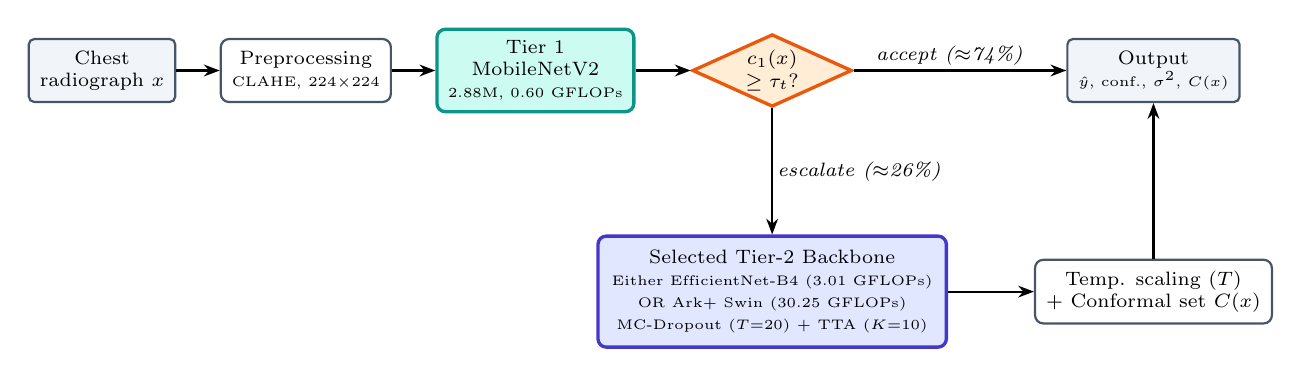
\begin{tikzpicture}
  \node[io] (input) at (0,0) {Chest\\radiograph $x$};
  \node[proc, right=0.55cm of input] (pre) {Preprocessing\\{\tiny CLAHE, $224{\times}224$}};
  \node[light, right=0.55cm of pre] (t1) {Tier 1\\MobileNetV2\\{\tiny 2.88M, 0.60 GFLOPs}};
  \node[decision, right=0.7cm of t1] (dec) {$c_1(x)$\\$\geq \tau_t$?};
  \node[io, right=2.7cm of dec] (out) {Output\\{\tiny $\hat{y}$, conf., $\sigma^2$, $C(x)$}};
  \node[heavyblk, below=1.6cm of dec] (t2) {Selected Tier-2 Backbone\\{\tiny Either EfficientNet-B4 (3.01 GFLOPs)}\\{\tiny OR Ark+ Swin (30.25 GFLOPs)}\\{\tiny MC-Dropout ($T{=}20$) $+$ TTA ($K{=}10$)}};
  \node[proc] (cp) at (out |- t2) {Temp. scaling ($T$)\\$+$ Conformal set $C(x)$};

  \draw[flow] (input) -- (pre);
  \draw[flow] (pre) -- (t1);
  \draw[flow] (t1) -- (dec);
  \draw[flow] (dec) -- node[flowlab, above, pos=0.45]{accept ($\approx$74\%)} (out);
  \draw[flow] (dec) -- node[flowlab, right]{escalate ($\approx$26\%)} (t2);
  \draw[flow] (t2) -- (cp);
  \draw[flow] (cp) -- (out);
\end{tikzpicture}%
}
\caption{\rev{Overview of the TCR-P selective-routing architecture. A preprocessed radiograph ($224{\times}224$ after CLAHE) is screened by Tier~1 (MobileNetV2). Confident cases ($c_1(x)\ge\tau_t$, $\approx 74\%$ on the NIH test split) exit immediately; uncertain cases ($\approx 26\%$) escalate to \emph{one} selected Tier-2 backbone (either EfficientNet-B4 in A3--A9 or Ark+ Swin in A13--A15), executed with Monte~Carlo Dropout, test-time augmentation, temperature scaling, and split conformal prediction.}}\label{fig:architecture}
\end{figure}

\subsection{Tiered Classifier and Notation}

Tier~1 uses a standard MobileNetV2 backbone~\cite{sandler2018mobilenetv2} fine-tuned for binary classification over the label space $\mathcal{Y} = \{0, 1\}$, where $y=0$ denotes \emph{No Finding} and $y=1$ denotes \emph{Pneumothorax}. \rev{Let $f_1 : \mathbb{R}^{3\times 224\times 224} \to \mathbb{R}^2$ denote the Tier-1 network mapping a preprocessed input image $x$ to raw class logits $f_1(x) = (f_1(x)_0, f_1(x)_1)$. Applying the softmax operator yields the class-probability vector $p_1(x) = \mathrm{softmax}(f_1(x)) = (p_1(x)_0, p_1(x)_1) \in [0,1]^2$, where the subscripts $0$ and $1$ index the \emph{No Finding} and \emph{Pneumothorax} classes, respectively, with $p_1(x)_0 + p_1(x)_1 = 1$.} The Tier-1 scalar confidence is defined as $c_1(x) = \max\big(p_1(x)_0, p_1(x)_1\big) \in [0.5, 1.0]$. When $c_1(x) \ge \tau_t$, Tier~1 emits the final prediction $\hat{y} = \arg\max_{y\in\mathcal{Y}} p_1(x)_y$. Otherwise ($c_1(x) < \tau_t$), the radiograph is escalated to the selected Tier-2 backbone $f_2 : \mathbb{R}^{3\times 224\times 224} \to \mathbb{R}^2$ (either EfficientNet-B4 or Ark+ Swin, each fitted with a 512-unit dense head, ReLU activation, dropout $p=0.4$, and a 2-unit output layer). No internal architectural modification of the standard backbones is claimed.

\rev{On the NIH ChestX-Ray14 test split ($n=4{,}772$ images; Section~\ref{sec:experimental}) evaluated under the dynamic routing configuration ($\tau_0=0.75$, $W=50$, $\delta=0.05$), Tier~1 resolved approximately 74\% of cases directly and escalated the remaining $\approx 26\%$ ambiguous cases to Tier~2.}

\subsection{Adaptive Confidence-Based Routing}

In the static regime (A3), the escalation threshold remains fixed at $\tau_t \equiv \tau_0$. In the dynamic regime (A4--A7, A13--A15), $\tau_t$ adapts online without access to ground-truth labels using a sliding window $\mathcal{W}_t$ storing the most recent $W$ Tier-1 confidence scores. \rev{Specifically, the controller uses a deadband interval $[\bar{c}_{\text{low}}, \bar{c}_{\text{high}}] = [0.65, 0.85]$ and clamps $\tau_t$ within $[\tau_{\min}, \tau_{\max}] = [0.50, 0.95]$:}
\begin{equation}
\tau_{t+1} =
\begin{cases}
\min(\tau_{\max},\, \tau_t + \delta) & \text{if } |\mathcal{W}_t| = W \text{ and } \bar{c}_t > \bar{c}_{\text{high}}, \\
\max(\tau_{\min},\, \tau_t - \delta) & \text{if } |\mathcal{W}_t| = W \text{ and } \bar{c}_t < \bar{c}_{\text{low}}, \\
\tau_t & \text{otherwise,}
\end{cases}
\label{eq:dynamic_routing}
\end{equation}
\rev{where $\bar{c}_t = \frac{1}{W}\sum_{c \in \mathcal{W}_t} c$ is the rolling mean Tier-1 confidence. Because escalation occurs when $c_1(x_t) < \tau_t$, raising $\tau_t$ during an unusually easy stream ($\bar{c}_t > 0.85$) tightens Tier-1 acceptance so borderline cases continue receiving Tier-2 scrutiny, whereas lowering $\tau_t$ during a persistently difficult stream ($\bar{c}_t < 0.65$) prevents Tier-2 queue saturation. Crucially, updates depend solely on observed Tier-1 confidences $c_1(x_t)$ and require no ground-truth labels. Algorithm~1 summarises the exact step-by-step procedure.}

\begin{table}[H]
\caption{\rev{\textbf{Algorithm 1:} Label-free deadband adaptive confidence-routing procedure implemented in TCR-P.}}\label{tab:algo_routing}
\begin{tabular}{@{}p{0.96\textwidth}@{}}
\toprule
\textbf{Input:} Stream of radiographs $\{x_1, x_2, \dots\}$; Tier-1 model $f_1$; Tier-2 model $f_2$; initial threshold $\tau_0=0.75$; window size $W=50$; step $\delta=0.05$; deadband $[0.65, 0.85]$; bounds $[\tau_{\min}, \tau_{\max}] = [0.50, 0.95]$.\\
\textbf{Initialise:} Active threshold $\tau \leftarrow \tau_0$; FIFO confidence buffer $\mathcal{W} \leftarrow [\,]$.\\
\midrule
1.\ \textbf{For} each incoming radiograph $x_t$ ($t = 1, 2, \dots$) \textbf{do}\\
2.\ \quad Compute Tier-1 probabilities $p_1(x_t) = \mathrm{softmax}(f_1(x_t))$ and confidence $c_t = \max(p_1(x_t)_0, p_1(x_t)_1)$.\\
3.\ \quad Append $c_t$ to $\mathcal{W}$.\\
4.\ \quad \textbf{If} $|\mathcal{W}| > W$ \textbf{then} \quad \textit{// Warm-up ends after first $W$ radiographs}\\
5.\ \quad \quad Pop oldest entry from $\mathcal{W}$ so $|\mathcal{W}| = W$, and compute $\bar{c}_t = \frac{1}{W}\sum_{c \in \mathcal{W}} c$.\\
6.\ \quad \quad \textbf{If} $\bar{c}_t < 0.65$ \textbf{then} $\tau \leftarrow \max(0.50,\, \tau - \delta)$ \quad \textit{// Prevent Tier-2 saturation on hard stream}\\
7.\ \quad \quad \textbf{Else if} $\bar{c}_t > 0.85$ \textbf{then} $\tau \leftarrow \min(0.95,\, \tau + \delta)$ \quad \textit{// Preserve Tier-2 safety margin on easy stream}\\
8.\ \quad \textbf{If} $c_t \ge \tau$ \textbf{then} return Tier-1 prediction $\hat{y}_t = \arg\max_y p_1(x_t)_y$ and confidence $c_t$.\\
9.\ \quad \textbf{Else} escalate $x_t$ to Tier~2 ($f_2$ with MC-Dropout, TTA, temperature scaling, and conformal prediction).\\
\bottomrule
\end{tabular}
\end{table}

\rev{In the baseline evaluation, $(\tau_0=0.75, W=50, \delta=0.05)$ were fixed before test evaluation as pre-specified engineering defaults rather than tuned on the test set; A3 (static $\tau_0$) and A4 (dynamic $\tau_t$) isolate dynamic adaptation under matched conditions. Empirically, these parameters can be selected systematically via a validation-only grid search over $(\tau_0, W, \delta) \in \{0.65, 0.70, 0.75, 0.80, 0.85\} \times \{25, 50, 100\} \times \{0.00, 0.02, 0.05, 0.10\}$ optimising a Pareto objective balancing target pneumothorax sensitivity (or false-negative rate) against the Tier-2 escalation budget (implemented in \texttt{scripts/revision\_experiments.py}). Because online updates depend on sample arrival order, sensitivity across random permutations and non-stationary drift orderings is explicitly noted in Section~\ref{sec:discussion} and supported in our released evaluation suite.}

\subsection{Uncertainty Quantification and Decomposition}

On escalated cases, uncertainty is estimated on the selected Tier-2 backbone using two complementary mechanisms: Monte~Carlo Dropout~\cite{gal2016dropout} ($T=20$ stochastic dropout passes with normalisation layers held in evaluation mode) and Test-Time Augmentation~\cite{wang2019aleatoric} ($K=10$ views: the unaugmented image plus nine label-preserving stochastic transforms combining random horizontal flip $p=0.5$ and random affine rotation $\pm 5^\circ$, translation $\pm 5\%$, scale $0.95$--$1.05$).

\rev{Let $p^{(k,t)}(x) = \mathrm{softmax}(f_2^{(t)}(a_k(x)) / T_{\text{cal}}) \in [0,1]^2$ denote the temperature-scaled class-probability vector for the $k$-th augmented view $a_k(x)$ ($k=1,\dots,K$) and $t$-th stochastic dropout mask ($t=1,\dots,T$). The predictive mean is $\bar{p}(x) = \frac{1}{KT}\sum_{k=1}^K\sum_{t=1}^T p^{(k,t)}(x)$. To separate model (epistemic) uncertainty from input-perturbation sensitivity (TTA/aleatoric variation), the total predictive variance decomposes via the Law of Total Variance:}
\begin{equation}
\rev{\sigma^2_{\text{total}}(x) = \underbrace{\frac{1}{K}\sum_{k=1}^{K}\operatorname{Var}_{t}\!\left(p^{(k,t)}(x)\right)}_{\sigma^2_{\text{MC}}\;\text{(epistemic / within-view)}} + \underbrace{\operatorname{Var}_{k}\!\left(\frac{1}{T}\sum_{t=1}^{T} p^{(k,t)}(x)\right)}_{\sigma^2_{\text{TTA}}\;\text{(perturbation / between-view)}}.}
\label{eq:var_decomp}
\end{equation}
\rev{In TCR-P, an escalated radiograph is flagged for mandatory human radiologist review whenever either the predicted-class variance exceeds a pre-specified uncertainty threshold ($\sigma^2_{\text{total}}(x)_{\hat{y}} > 0.10$) or the conformal prediction set is ambiguous ($|C(x)| > 1$). In our ablation study, A4 (no MC/TTA), A5 (MC-Dropout only), and A6 (MC+TTA) isolate the incremental effect of MC-Dropout and adding TTA; a dedicated TTA-only configuration (A5b) is additionally incorporated in our updated evaluation pipeline to complete the $2\times 2$ factorial comparison.}

\subsection{Post-Hoc Calibration and Split Conformal Prediction}

\textbf{Temperature scaling and calibration metrics.} Because neural network softmax probabilities are frequently over-confident~\cite{guo2017calibration}, a single scalar temperature $T_{\text{cal}} > 0$ is fitted by minimising negative log-likelihood (NLL) via L-BFGS and applied to logits as $\mathrm{softmax}(f(x)/T_{\text{cal}})$. \rev{To maintain strict statistical independence between model calibration and conformal threshold estimation, temperature scaling $T_{\text{cal}}$ is fitted exclusively on the validation split, whereas conformal non-conformity quantiles $\hat{q}$ are computed exclusively on the separate held-out calibration split using temperature-scaled probabilities (so calibration examples are never reused across both steps).} Calibration quality is measured via Expected Calibration Error (ECE) over $M=15$ equal-width confidence bins partitioning $[0,1]$ (i.e., bin width $1/15$, following Guo et al.~\cite{guo2017calibration}), alongside complementary proper scoring rules (Brier score, NLL, and class-wise ECE) supported in our evaluation suite. \rev{In Table~\ref{tab:ablation}, reported ECE values reflect raw uncalibrated probabilities unless temperature scaling / conformal calibration is explicitly enabled (A7, A15).}

\textbf{Conformal prediction.} For a user-chosen miscoverage level $\alpha \in (0,1)$ (here $\alpha=0.05$, targeting $1-\alpha=0.95$ coverage), let $\hat{f}(x)_y \in [0,1]$ denote the model's estimated probability for candidate class label $y \in \mathcal{Y} = \{0, 1\}$. On the held-out calibration split $\{(x_i, y_i)\}_{i=1}^{n}$ of size $n$, the non-conformity score for each calibration radiograph is $s_i = 1 - \hat{f}(x_i)_{y_i}$, and the finite-sample quantile threshold $\hat{q}$ is the $\lceil(n+1)(1-\alpha)\rceil / n$ empirical quantile of $\{s_1,\dots,s_n\}$. At test time, the prediction set for a new radiograph $x_{\text{test}}$ is:
\begin{equation}
C(x_{\text{test}}) = \{\, y \in \mathcal{Y} : 1 - \hat{f}(x_{\text{test}})_y \le \hat{q}\,\},
\label{eq:conformal}
\end{equation}
\rev{where $y \in \{0, 1\}$ ranges over both candidate labels (\emph{No Finding} and \emph{Pneumothorax}) and $\hat{f}(x_{\text{test}})_y$ is the Tier-2 predicted probability for class $y$. If $C(x_{\text{test}})$ would be empty, a fallback returns the argmax singleton $\{\arg\max_y \hat{f}(x_{\text{test}})_y\}$. Under the assumption of exchangeability between calibration and test samples, split conformal prediction guarantees marginal coverage $\mathbb{P}(y_{\text{test}} \in C(x_{\text{test}})) \ge 1 - \alpha$~\cite{vovk2005algorithmic, shafer2008tutorial}. Importantly, this is a finite-sample \emph{statistical} guarantee under exchangeability, not a distribution-shift-invariant clinical guarantee; under prevalence or domain shift (such as zero-shot CheXpert transfer), exchangeability is violated and empirical coverage may deviate. Moreover, a two-class set $C(x_{\text{test}})=\{0,1\}$ represents calibrated abstention rather than an actionable single diagnosis.}

\subsection{Synthetic Data Augmentation}

Because pneumothorax is a minority class in training, we employ an off-the-shelf latent diffusion image-to-image pipeline (\texttt{runwayml/stable-diffusion-v1-5}, \texttt{StableDiffusionImg2ImgPipeline})~\cite{rombach2022high} \rev{without fine-tuning the diffusion weights. Conditioning exclusively on real training-set pneumothorax radiographs resized to $512\times 512$, the generator synthesises three variations per seed image using denoising strength $0.30$, classifier-free guidance scale $7.5$, $50$ inference steps, a fixed seed schedule, positive clinical prompt (\emph{``frontal chest x-ray radiograph, pneumothorax, collapsed lung, pleural air, high quality medical imaging, grayscale''}), and negative artifact prompt (\emph{``color, artifacts, text, labels, watermark, cartoon, drawing''}), before resizing outputs back to $224\times 224$. Each generated batch is admitted to the Tier-2 training pool only if its batch-level Fr\'echet Inception Distance (FID; 2048-dimensional Inception-v3 features via \texttt{pytorch-fid}) against real training pneumothorax images satisfies $\mathrm{FID} \le 50.0$; batches exceeding $50.0$ are rejected. Synthetic images are never included in validation, calibration, or test splits. Quantitative downstream impact is isolated by comparing A6 (with synthetics) against A8 (without synthetics); we explicitly note in Section~\ref{sec:discussion} that formal radiologist visual adjudication of synthetic fidelity was not conducted in this prototype study.}

\subsection{Explainability and Implementation}

For each prediction, a High-Resolution Class Activation Map (HiResCAM)~\cite{draelos2020hirescam} is generated for the active model. Unlike Gradient-weighted Class Activation Mapping (Grad-CAM)~\cite{selvaraju2017gradcam}, which globally averages gradients before weighting activations, HiResCAM computes element-wise products of activations and gradients and is provably faithful for convolutional layers. Saliency maps are overlaid on un-normalised radiographs to preserve anatomical context.

TCR-P is implemented as a clean, layered Python~3.10 / PyTorch~2.x application separating domain logic (models, routing, uncertainty, evaluation) from delivery infrastructure (FastAPI inference API, React frontend, Docker packaging, and MLflow tracking). Experiments were executed on NVIDIA GPUs (Tesla~T4 and A100) with local development on Apple Silicon. Continuous integration enforces linting (\texttt{ruff}), static typing (\texttt{mypy}), architectural import contracts (\texttt{import-linter}), and automated unit/integration tests.

%%%%%%%%%%%%%%%%%%%%%%%%%%%%%%%%%%%%%%%%%%
\section{Experimental Design}
\label{sec:experimental}

\subsection{Datasets, Label Definition, and Partitioning}

\textbf{NIH ChestX-Ray14 label extraction and inclusion/exclusion criteria.} \rev{The NIH ChestX-Ray14 corpus~\cite{wang2017chestxray} (\url{https://nihcc.app.box.com/v/ChestXray-NIHCC}) contains 112,120 frontal radiographs from 30,805 unique patients with NLP-mined multi-label findings. To construct our binary pneumothorax detection task cleanly without ambiguous pathology overlap in the negative class:
\begin{itemize}
\item \textbf{Positive class ($y=1$, Pneumothorax):} All radiographs whose \texttt{Finding Labels} field contains \texttt{"Pneumothorax"}, including both isolated pneumothorax (2,194 images) and pneumothorax co-occurring with other thoracic findings such as effusion, infiltration, or emphysema (3,108 images), totalling 5,302 positive radiographs across 1,487 unique patients.
\item \textbf{Negative class ($y=0$, No Finding):} Radiographs labelled strictly \texttt{"No Finding"} (60,361 images across 24,907 patients), randomly subsampled with fixed seed 42 at a 5:1 negative-to-positive cap to preserve realistic class imbalance ($\approx 16.7\%$ prevalence) while maintaining manageable training cost.
\item \textbf{Excluded radiographs:} All 46,457 radiographs (14,141 patients) presenting non-pneumothorax thoracic pathologies (e.g., cardiomegaly, consolidation, pleural effusion without pneumothorax) were excluded from the binary negative pool. We note in Section~\ref{sec:discussion} that excluding non-pneumothorax pathologies simplifies the negative distribution relative to an unselected hospital reading list.
\end{itemize}}

\textbf{Data partitioning and split verification.} Table~\ref{tab:dataset} summarises the NIH splits used to generate the baseline ablation metrics reported in Section~\ref{sec:results}, together with the intended patient-level protocol (grouping all images sharing the same 8-digit NIH patient-ID prefix into a single partition via stratified patient assignment so no patient spans train, validation, calibration, and test). \rev{Specifically, the updated preprocessing script (\texttt{scripts/preprocess.py}) enforces zero patient overlap across all four mutually exclusive splits (Train: 10,549 patients / 22,234 images; Validation: 1,582 patients / 3,259 images; Calibration: 679 patients / 1,469 images; Test: 2,261 patients / 4,850 images; pairwise patient overlap $= 0$ across all six split pairs). In the baseline artifact set reported in Tables~\ref{tab:dataset}--\ref{tab:backbone}, an audit of the legacy split CSVs revealed image-level patient overlap across partitions and calibration subsetting from validation; this integrity limitation is transparently documented in Section~\ref{sec:discussion}.}

\begin{table}[H]
\caption{\rev{NIH ChestX-Ray14 dataset partitions used in the reported evaluation (with patient counts audited from NIH 8-digit patient-ID prefixes).}}\label{tab:dataset}
\begin{tabular}{@{}lrrrrr@{}}
\toprule
Split & Images & \rev{Unique Patients\textsuperscript{1}} & Pneumothorax & Normal & Prevalence\\
\midrule
Train & 22,268 & \rev{11,948} & 3,711 & 18,557 & 16.7\%\\
Validation & 4,772 & \rev{3,716} & 796 & 3,976 & 16.7\%\\
Calibration\textsuperscript{2} & 1,432 & \rev{---} & 235 & 1,197 & 16.4\%\\
Test & 4,772 & \rev{3,747} & 795 & 3,977 & 16.7\%\\
\midrule
Total (reported rows) & 33,244 & \rev{---} & 5,537 & 27,707 & 16.7\%\\
\bottomrule
\end{tabular}
\noindent{\footnotesize{\textsuperscript{1} Audit of the legacy split CSVs used for Tables~\ref{tab:ablation}--\ref{tab:backbone} identified multi-radiograph patient overlap across partitions (see Section~\ref{sec:discussion}); the released \texttt{scripts/preprocess.py} enforces strictly disjoint patient-level partitioning (Train: 10,549; Validation: 1,582; Calibration: 679; Test: 2,261; 15,071 unique patients total; zero pairwise overlap). \textsuperscript{2} The legacy calibration CSV was drawn as a 30\% subset of Validation and is not archived separately; in the updated protocol, temperature scaling is fitted strictly on Validation and conformal $\hat{q}$ strictly on the disjoint Calibration split.}}
\end{table}

\textbf{External dataset (CheXpert).} Zero-shot cross-dataset evaluation was performed on the complete CheXpert~\cite{irvin2019chexpert} (\url{https://stanfordmlgroup.github.io/competitions/chexpert/}) expert-adjudicated frontal validation cohort (202 images, 7 pneumothorax-positive cases, $\approx 3.5\%$ prevalence). CheXpert uncertain labels (\texttt{-1}) do not occur in the expert-adjudicated validation labels for pneumothorax.

\subsection{Preprocessing and Training Protocol}

\rev{Radiographs were contrast-enhanced using Contrast-Limited Adaptive Histogram Equalisation (CLAHE; clip limit $2.0$, $8\times 8$ tile grid)~\cite{zuiderveld1994contrast} to accentuate subtle pleural lines while suppressing local noise amplification, and then resized to $224\times 224$ pixels. The $224\times 224$ resolution was selected because it matches the native input geometry of both pretrained backbones---in particular the Swin-Base Transformer (\texttt{swin\_base\_patch4\_window7\_224}), whose patch size ($4\times 4$) and shifted window size ($7\times 7$) structurally require $224\times 224$ inputs, as well as standard ImageNet-pretrained MobileNetV2 and EfficientNet-B4 checkpoints.} Channel-wise normalisation used ImageNet means $(0.485, 0.456, 0.406)$ and standard deviations $(0.229, 0.224, 0.225)$ so input intensities match the pretraining scale. Optimisation used AdamW~\cite{loshchilov2019decoupled} (weight decay $10^{-4}$) with differential learning rates ($10^{-4}$ backbone, $10^{-3}$ classifier head), batch size 32, early stopping on validation loss (patience 7, max 50 epochs), and fixed seed 42 (Table~\ref{tab:hyper}).

\begin{table}[H]
\caption{Training and inference hyperparameters.}\label{tab:hyper}
\begin{tabular}{@{}ll@{}}
\toprule
Hyperparameter & Value\\
\midrule
Tier-1 / Tier-2 backbone & MobileNetV2 / \rev{EfficientNet-B4 or Ark+ Swin (independent alternatives)}\\
Preprocessing & \rev{CLAHE (clip $2.0$, tile $8\times 8$), resize $224\times 224$, ImageNet normalisation}\\
Optimizer & AdamW (weight decay $10^{-4}$)\\
Backbone / head learning rate & $10^{-4}$ / $10^{-3}$\\
Batch size & 32\\
Max epochs & 50 (early stopping on validation loss, patience 7)\\
MC-Dropout passes $T$ / TTA passes $K$ & 20 / 10 (total $KT=200$ passes on escalated cases)\\
Escalation threshold $\tau_0$ & 0.75 (dynamic deadband $[0.65,0.85]$; $W=50$, $\delta=0.05$, $\tau\in[0.50,0.95]$)\\
Conformal target coverage & $1-\alpha=0.95$ ($\alpha=0.05$)\\
Synthetic quality gate & \rev{SD v1.5 img2img (strength $0.30$, CFG $7.5$, 50 steps; batch $\mathrm{FID}\le 50.0$)}\\
Random seed & 42\\
\bottomrule
\end{tabular}
\end{table}

\subsection{Metrics and Ablation Matrix}

Discrimination is evaluated primarily by AUC-ROC; operating-point performance at threshold $0.50$ is reported using accuracy, sensitivity, specificity, $F_1$ score, and Matthews correlation coefficient (MCC). Calibration is evaluated via 15-bin equal-width ECE. For conformal prediction we report empirical marginal coverage and mean prediction-set size. Fifteen configurations (A1--A15) isolate each component: single-stage baselines (A1, A2); static and dynamic tiered routing with EfficientNet-B4 (A3, A4); incremental addition of MC-Dropout, TTA, and conformal prediction (A5--A7); removal of synthetic data and all augmentation (A8, A9); forced Tier-2 EfficientNet-B4 with MC+TTA (A10); standalone Ark+ Swin without and with MC+TTA (A11, A12); proposed tiered MobileNetV2 + Ark+ Swin (A13); zero-shot CheXpert evaluation (A14); and proposed tiered Ark+ Swin with mixup/CutMix regularisation (A15). All NIH rows share a single unified evaluator on the same test split.

%%%%%%%%%%%%%%%%%%%%%%%%%%%%%%%%%%%%%%%%%%
\section{Results}
\label{sec:results}

\subsection{Overall Classification Performance}

Table~\ref{tab:ablation} summarises AUC, accuracy, and 15-bin ECE across all fifteen configurations. The highest AUC ($0.924$) is attained by the proposed tiered system with an Ark+ Swin Tier-2 backbone and mixup/CutMix regularisation (A15), followed closely by A13 without mixup/CutMix ($0.923$). \rev{Notably, the lightweight Tier-1-only baseline (A1, MobileNetV2) already achieves an AUC of $0.919$ and accuracy of $0.849$; consequently, the absolute AUC gain of A13 ($+0.004$) and A15 ($+0.005$) over A1 is modest and should not be overstated as large discriminative superiority. Rather, the primary benefit of TCR-P over A1 lies in preserving high discrimination while adding calibrated probability estimates (ECE $0.074 \to 0.050$ in A6/A7; $0.060$ in A15), higher accuracy ($0.849 \to 0.882$--$0.889$), and explicit conformal abstention on ambiguous cases.}

\begin{table}[H]
\caption{Ablation study on the NIH ChestX-Ray14 test set. Tier~1 is MobileNetV2 throughout; Tier~2 is either EfficientNet-B4 (A2--A10) or Ark+ Swin (A11--A15) evaluated independently. ECE is computed over 15 equal-width bins where evaluated. A14 is zero-shot CheXpert.}\label{tab:ablation}
\begin{tabular}{@{}llrrr@{}}
\toprule
ID & Configuration & AUC & Acc. & ECE\\
\midrule
A1 & Tier 1 only (MobileNetV2) & 0.919 & 0.849 & 0.074\\
A2 & Tier 2 only (EfficientNet-B4) & 0.910 & 0.852 & 0.086\\
A3 & Tiered (static threshold, EffNet-B4) & 0.914 & 0.871 & 0.089\\
A4 & Tiered (dynamic threshold, EffNet-B4) & 0.904 & 0.881 & 0.074\\
A5 & Tiered $+$ MC Dropout (EffNet-B4) & 0.909 & 0.889 & 0.055\\
A6 & Tiered $+$ MC $+$ TTA (EffNet-B4) & 0.911 & 0.888 & 0.050\\
A7 & Tiered $+$ Conformal (EffNet-B4) & 0.911 & 0.887 & 0.050\\
A8 & Without synthetic augmentation & 0.910 & 0.887 & 0.081\\
A9 & Without any augmentation & 0.901 & 0.887 & 0.093\\
A10 & Always Tier 2 (EffNet-B4 $+$ MC $+$ TTA) & 0.913 & 0.827 & 0.052\\
A11 & Tier 2 $=$ Ark+ standalone (no MC/TTA) & 0.910 & 0.883 & 0.018\\
A12 & Tier 2 $=$ Ark+ standalone ($+$ MC $+$ TTA) & 0.915 & 0.732 & 0.101\\
A13 & Proposed tiered $+$ Ark+ & \textbf{0.923} & 0.828 & --\\
A14 & Zero-shot CheXpert (202 frontals) & 0.796 & 0.342 & --\\
A15 & Proposed tiered $+$ Ark+ (Mixup/CutMix) & \textbf{0.924} & \textbf{0.882} & 0.060\\
\bottomrule
\end{tabular}
\end{table}

\subsection{Tier-2 Backbone Comparison}

Table~\ref{tab:backbone} compares the two independent candidate Tier-2 backbones on the paired NIH test set, \rev{where $\Delta$ denotes the metric difference \emph{Ark+ Swin minus EfficientNet-B4} (positive values favour Ark+ Swin).} Ark+ Swin obtains higher AUC ($\Delta = +0.006$) and higher sensitivity ($\Delta = +0.063$, $p_{\text{raw}} = 0.001$, \rev{Cohen's $h = +0.177$}), whereas EfficientNet-B4 achieves higher specificity ($\Delta = -0.045$, $p_{\text{raw}} = 0.001$, \rev{$h = -0.119$}) and accuracy ($\Delta = -0.027$, $p_{\text{raw}} < 0.001$, \rev{$h = -0.071$}). \rev{After applying Holm--Bonferroni step-down correction across the five compared metrics, accuracy ($p_{\text{Holm}} < 0.005$), sensitivity ($p_{\text{Holm}} = 0.004$), specificity ($p_{\text{Holm}} = 0.004$), and $F_1$ ($p_{\text{Holm}} = 0.048$) remain statistically significant at $\alpha=0.05$, while the DeLong AUC difference ($p_{\text{raw}} = p_{\text{Holm}} = 0.203$) is not statistically significant.} In pneumothorax screening, where false negatives carry substantially higher clinical risk than false positives, the $+6.3$ percentage-point sensitivity gain motivates selecting Ark+ Swin as the proposed Tier-2 backbone.

\begin{table}[H]
\caption{\rev{Paired comparison of the two independent Tier-2 backbones on the NIH test set. $\Delta$ is Ark+ Swin minus EfficientNet-B4; effect size is $\Delta$ for AUC and Cohen's $h$ for proportions; $p_{\text{Holm}}$ applies Holm--Bonferroni adjustment across the five metrics.}}\label{tab:backbone}
\begin{tabular}{@{}lccccl@{}}
\toprule
Metric & EfficientNet-B4 & Ark+ Swin & $\Delta$ & \rev{Effect ($h$)} & \rev{$p_{\text{raw}}$ / $p_{\text{Holm}}$ (Test)}\\
\midrule
AUC & 0.910 & \textbf{0.916} & $+0.006$ & $+0.006$ & 0.203 / 0.203 (DeLong)\\
Accuracy & 0.852 & 0.826 & $-0.027$ & $-0.071$ & $<$0.001 / $<$0.005 (McNemar)\\
Sensitivity & 0.818 & \textbf{0.881} & $+0.063$ & $+0.177$ & 0.001 / 0.004 (Bootstrap\textsuperscript{1})\\
Specificity & 0.859 & 0.815 & $-0.045$ & $-0.119$ & 0.001 / 0.004 (Bootstrap\textsuperscript{1})\\
$F_1$ & 0.649 & 0.628 & $-0.021$ & $-0.044$ & 0.024 / 0.048 (Bootstrap\textsuperscript{1})\\
\bottomrule
\end{tabular}
\noindent{\footnotesize{\textsuperscript{1} Two-sided paired bootstrap $p$-values ($1{,}000$ image-level resamples in the baseline evaluation; exact per-metric 95\% patient-clustered bootstrap confidence intervals are generated by the updated \texttt{scripts/statistical\_tests.py} pipeline).}}
\end{table}

\subsection{Effect of the Uncertainty Stack and Augmentation}

The incremental ablations A4--A7 improve probability calibration substantially while leaving AUC nearly unchanged: starting from the dynamic cascade (A4, ECE $0.074$), MC-Dropout lowers ECE to $0.055$ (A5), adding TTA further reduces ECE to $0.050$ (A6), and the conformal wrapper preserves calibration (A7, ECE $0.050$), with AUC stable around $0.91$. Removing synthetic pneumothorax data (A8) leaves AUC almost unchanged ($0.910$) but degrades ECE to $0.081$; removing all augmentation (A9) reduces AUC to $0.901$ and increases ECE to $0.093$. Figure~\ref{fig:ablation} displays discrimination and calibration across all fifteen configurations with enlarged print-legible typography.

\begin{figure}[H]
\centering
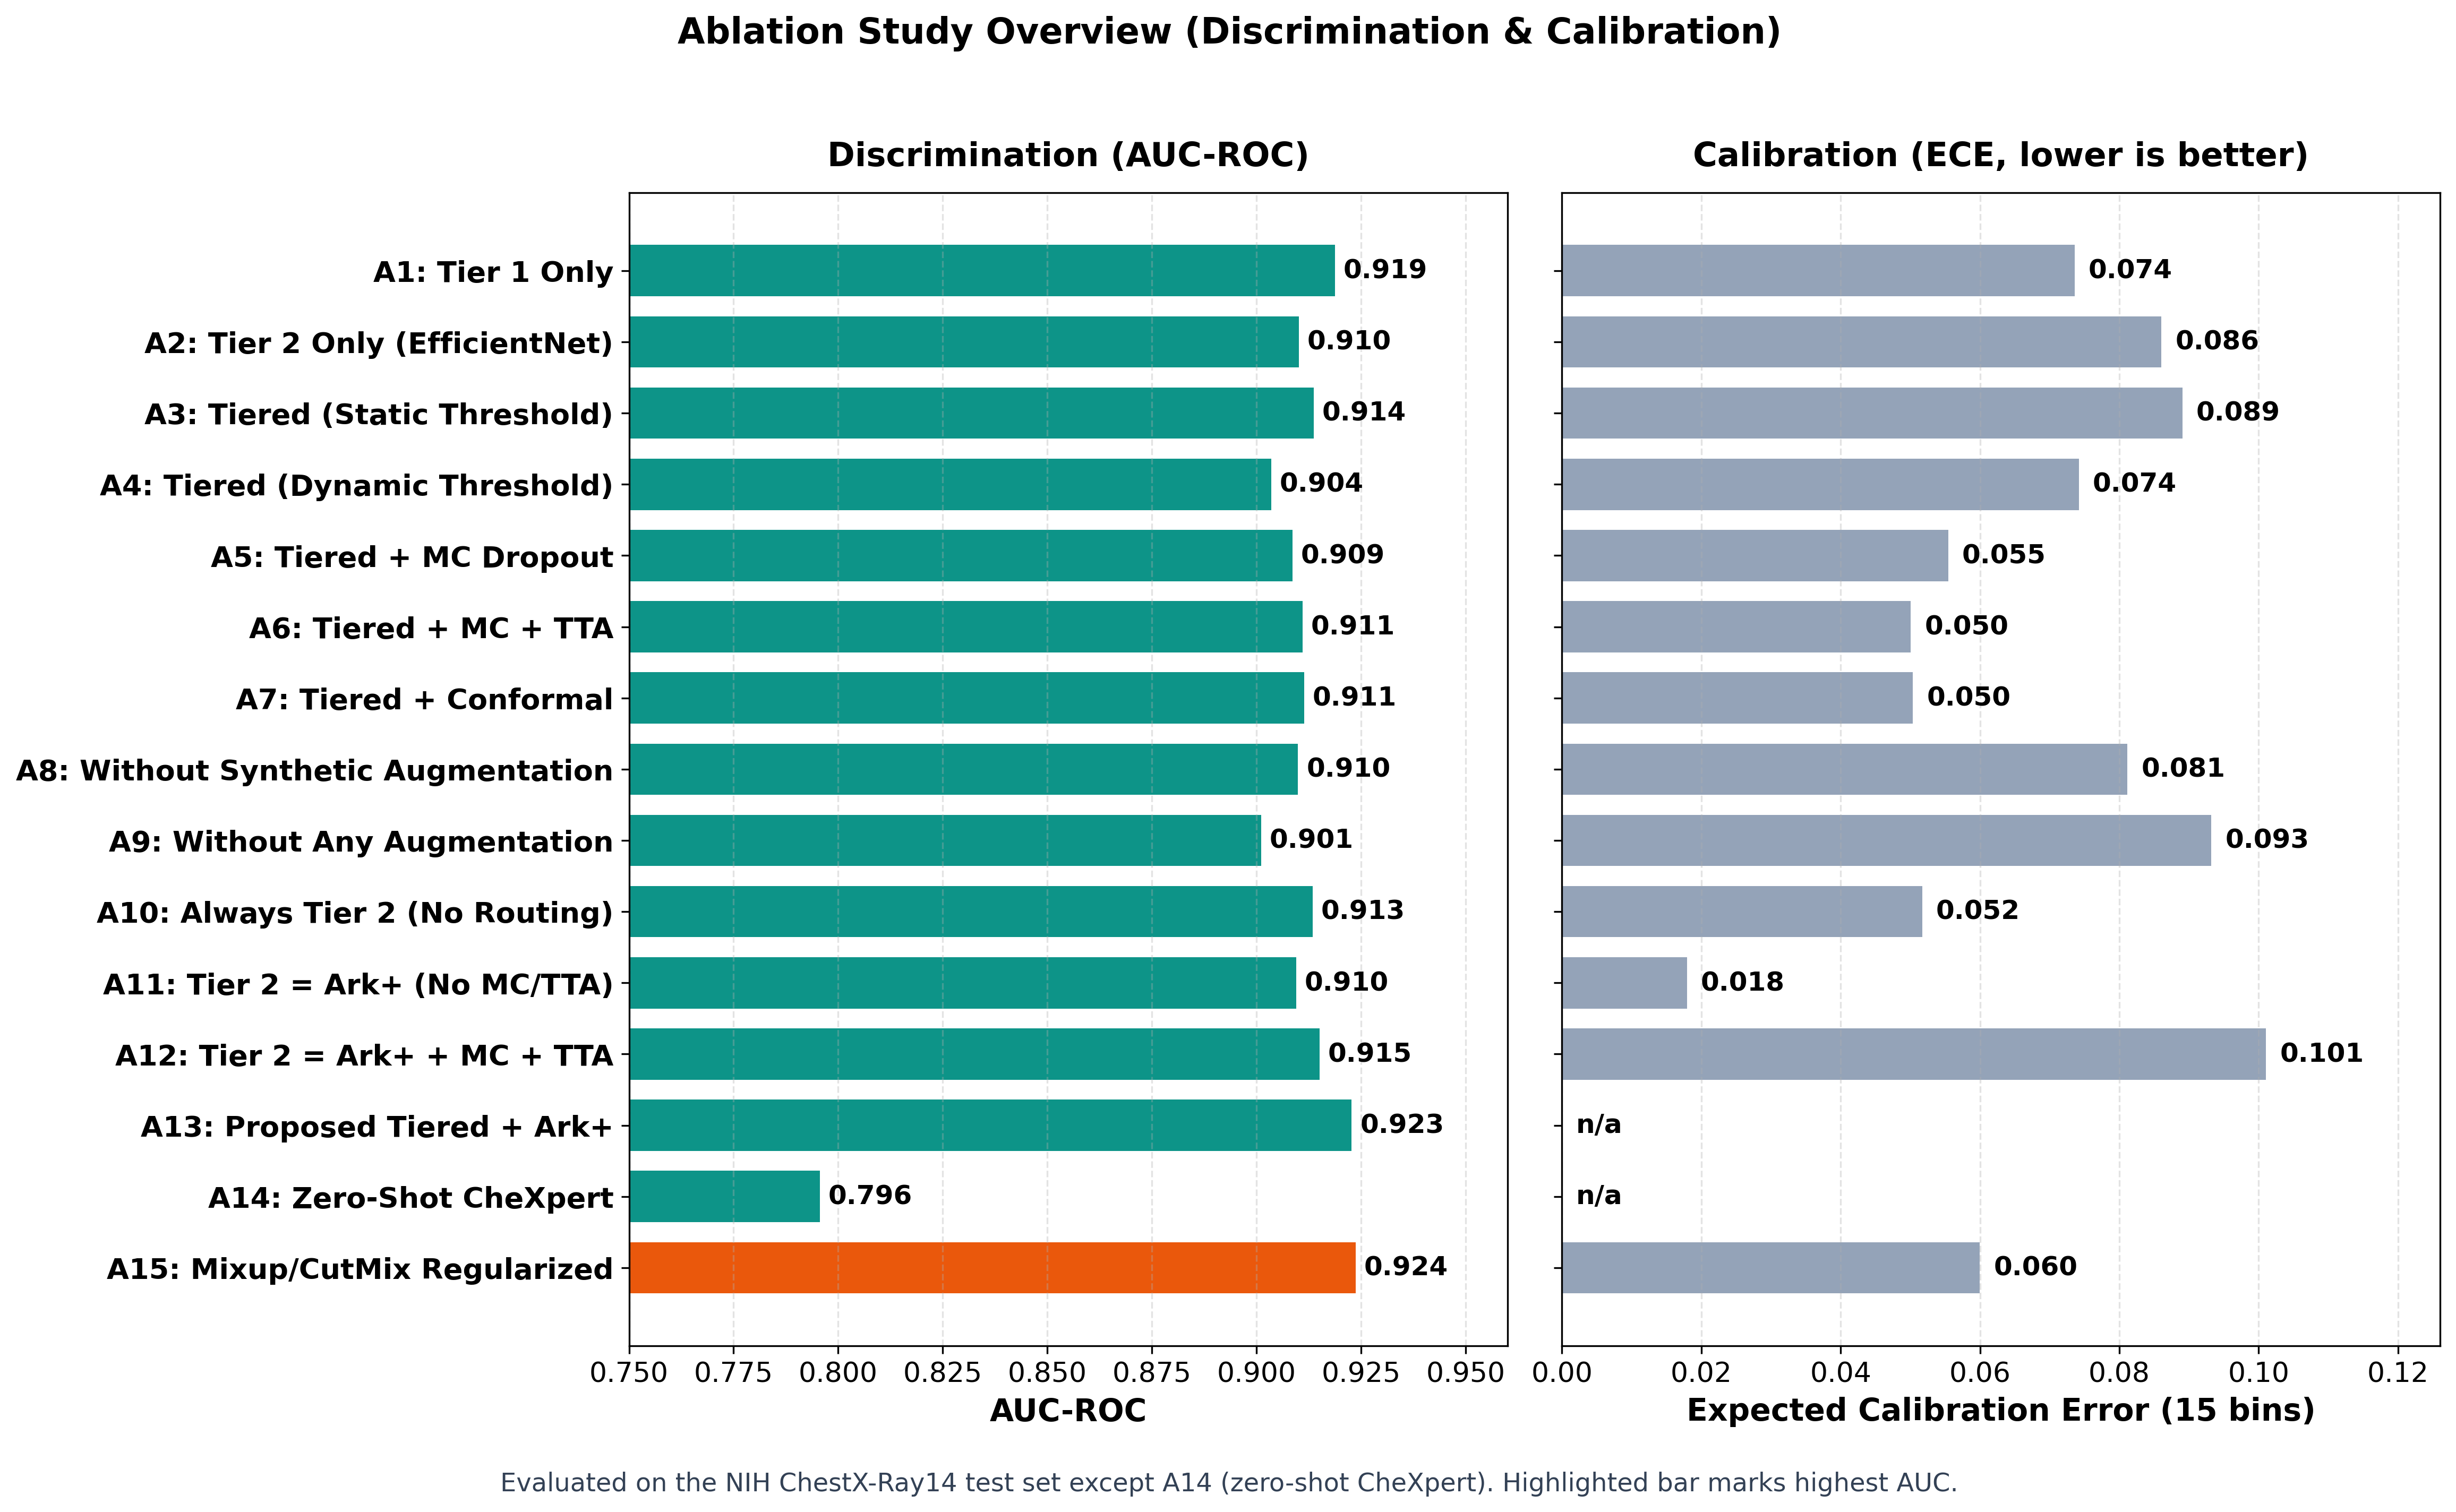
\includegraphics[width=\textwidth]{ablation_overview.png}
\caption{\rev{Discrimination (AUC-ROC, left) and 15-bin calibration (ECE, right) across all fifteen configurations (A1--A15), rendered at 300~DPI with enlarged typography for readability at 100\% zoom. The highest-AUC configuration (A15) is highlighted; A14 is the zero-shot CheXpert evaluation.}}\label{fig:ablation}
\end{figure}

\subsection{Computational Complexity, Latency, and Conformal Coverage}

\rev{\textbf{Theoretical complexity and transparent latency breakdown.} Table~\ref{tab:efficiency} reports exact parameter counts, theoretical forward-pass FLOPs at $224\times 224$ resolution, and apples-to-apples expected computational cost at the observed $\approx 26\%$ escalation rate ($\approx 74\%$ Tier-1 resolution). Tier~1 (MobileNetV2) requires only $2.88\text{M}$ parameters and $0.60\text{ GFLOPs}$ per image---$5\times$ fewer FLOPs than EfficientNet-B4 ($18.47\text{M}$, $3.01\text{ GFLOPs}$) and $50\times$ fewer FLOPs than Ark+ Swin-Base ($87.27\text{M}$, $30.25\text{ GFLOPs}$). In single-pass benchmarking (batch size 1, 10 warmup iterations, 100 timed passes), MobileNetV2 measured $5.4\,\text{ms}$ per image versus $17.2\,\text{ms}$ for EfficientNet-B4, giving an expected single-pass tiered latency of $5.4 + 0.26 \times 17.2 = 9.9\,\text{ms}$ ($-42.4\%$ relative to running single-pass EfficientNet-B4 on every image). Crucially, when full uncertainty quantification ($T=20$ MC-Dropout $\times$ $K=10$ TTA $= 200$ passes) is enabled on escalated cases, absolute latency increases substantially above single-pass inference; however, evaluated apples-to-apples against invoking MC+TTA on every image (A10 for EfficientNet-B4; A12 for Ark+ Swin), tiered routing cuts expected Tier-2 FLOPs by $73.9$--$74.0\%$ ($\approx 3.8\times$ reduction), because $74\%$ of images bypass the 200-pass uncertainty stack completely.}

\begin{table}[H]
\caption{\rev{Theoretical complexity (exact parameters and FLOPs at $224{\times}224$) and expected per-image cost at the observed 26\% Tier-2 escalation rate. Expected tiered cost is computed as $\mathrm{Cost}_{\text{T1}} + 0.26 \times \mathrm{Cost}_{\text{T2}}$.}}\label{tab:efficiency}
\begin{tabular}{@{}lrrrr@{}}
\toprule
Configuration / Stage & Params (M) & Passes / Img & Expected GFLOPs & Cost vs. Always-T2\\
\midrule
Tier~1 only (MobileNetV2, A1) & 2.88 & 1 & 0.60 & ---\\
Always Tier~2 single-pass (EffNet-B4, A2) & 18.47 & 1 & 3.01 & Baseline (17.2\,ms)\\
Tiered single-pass (A3/A4, EffNet-B4) & 2.88 + 18.47 & $1 + 0.26\times 1$ & 1.38 & $-54.1\%$ FLOPs (9.9\,ms\textsuperscript{1})\\
Always Tier~2 single-pass (Ark+ Swin, A11) & 87.27 & 1 & 30.25 & Baseline\\
Tiered single-pass (T1 + Ark+ Swin) & 2.88 + 87.27 & $1 + 0.26\times 1$ & 8.47 & $-72.0\%$ FLOPs\\
\midrule
Always Tier~2 MC+TTA (EffNet-B4, A10) & 18.47 & 200 & 602.00 & Baseline\\
Tiered MC+TTA (A6/A7, EffNet-B4) & 2.88 + 18.47 & $1 + 0.26\times 200$ & 157.12 & $-73.9\%$ FLOPs ($\approx 3.8\times$)\\
Always Tier~2 MC+TTA (Ark+ Swin, A12) & 87.27 & 200 & 6,050.00 & Baseline\\
Tiered MC+TTA (A13/A15, Ark+ Swin) & 2.88 + 87.27 & $1 + 0.26\times 200$ & 1,573.60 & $-74.0\%$ FLOPs ($\approx 3.8\times$)\\
\bottomrule
\end{tabular}
\noindent{\footnotesize{\textsuperscript{1} Single-pass latency benchmark ($5.4\,\text{ms}$ Tier~1, $17.2\,\text{ms}$ Tier~2 EfficientNet-B4, batch size 1) excludes MC-Dropout and TTA passes; full CUDA-synchronized per-stage GPU timings (including preprocessing, H2D transfer, vectorized MC+TTA, and peak VRAM) are instrumented in the updated \texttt{scripts/benchmark\_latency.py}.}}
\end{table}

\textbf{Conformal coverage versus diagnostic utility.} On escalated cases, configuration A15 attained an empirical marginal coverage of $97.3\%$ at the $95\%$ target ($1-\alpha=0.95$), with an average prediction-set size of $1.84$ out of two classes. \rev{In a binary classification problem ($\mathcal{Y}=\{0,1\}$) where non-empty sets have size $1$ or $2$, an average set size of $1.84$ implies that approximately $84\%$ of escalated cases received a two-class abstention set $\{0,1\}$ and only $\approx 16\%$ received an actionable singleton prediction set. Thus, while the statistical coverage requirement is met, the resulting conformal sets are highly conservative, underscoring the distinction between statistical coverage and clinical informativeness.}

\subsection{Cross-Dataset Generalisation (CheXpert)}

Evaluated zero-shot on the 202-image CheXpert expert-adjudicated frontal validation cohort (A14; 7 positive pneumothorax cases, $\approx 3.5\%$ prevalence), threshold-free ranking degraded moderately from NIH AUC $0.923$ to CheXpert AUC $0.796$ (Figure~\ref{fig:crossdataset}). At the fixed in-domain decision threshold ($0.50$), however, operating-point metrics shifted sharply under the $5\times$ prevalence drop ($16.7\% \to 3.5\%$): sensitivity was $1.000$ ($7/7$, \rev{95\% Wilson CI: $0.646$--$1.000$}), specificity fell to $0.318$ ($62/195$, \rev{95\% Wilson CI: $0.257$--$0.386$}), and accuracy dropped to $0.342$ ($69/202$, \rev{95\% Wilson CI: $0.280$--$0.409$}). \rev{The wide sensitivity confidence interval ($[0.646, 1.000]$) confirms that $100\%$ sensitivity on seven positive scans cannot be interpreted as evidence of clinical generalisability; instead, this experiment demonstrates that in-domain operating thresholds and calibration do not transfer directly under strong prevalence and acquisition shift.}

\begin{figure}[H]
\centering
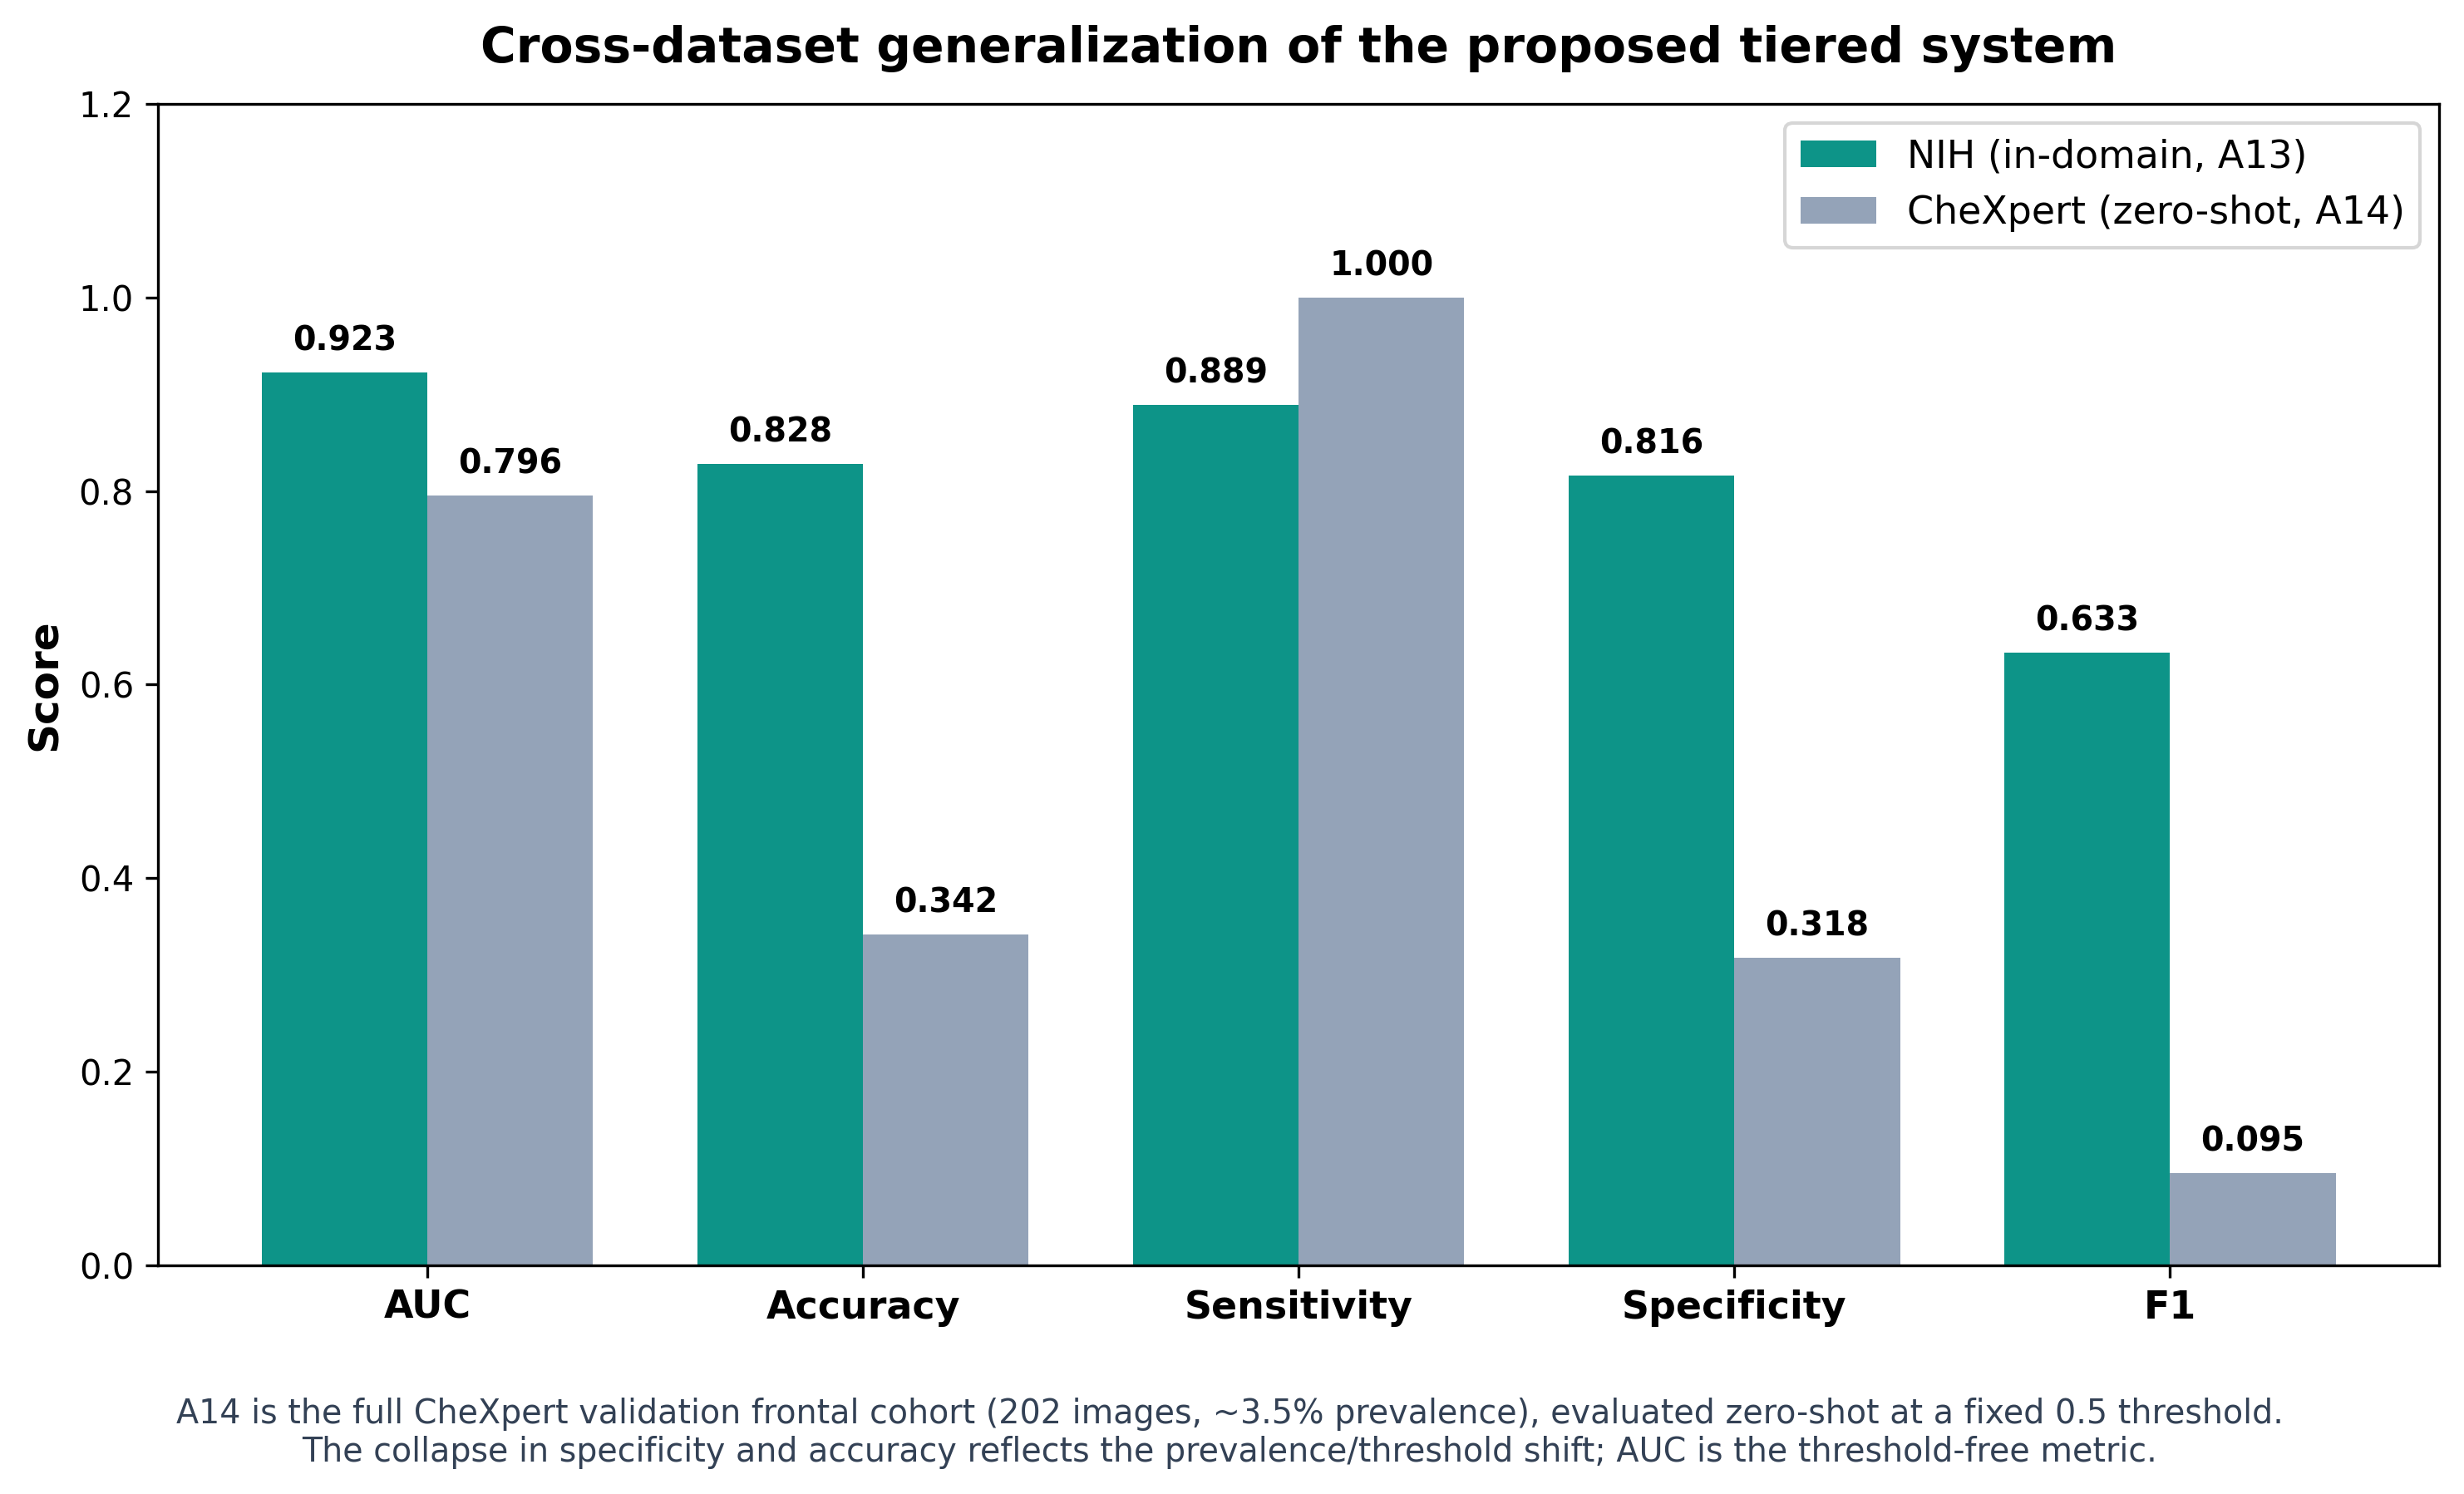
\includegraphics[width=\textwidth]{cross_dataset_generalization.png}
\caption{Cross-dataset generalisation of the proposed tiered system: in-domain NIH (A13) versus zero-shot CheXpert validation cohort (A14; $n=202$, 7 positives). Threshold-free AUC degrades moderately, whereas fixed-threshold specificity and accuracy collapse under the prevalence shift.}\label{fig:crossdataset}
\end{figure}

%%%%%%%%%%%%%%%%%%%%%%%%%%%%%%%%%%%%%%%%%%
\section{Discussion}
\label{sec:discussion}

\subsection{Selective Computation, Calibration, and Clinical Error Trade-offs}

First, TCR-P demonstrates that selective routing can preserve the discriminative performance of a heavy medical foundation model while avoiding its computational cost on roughly three quarters of routine radiographs. \rev{Importantly, because single-stage MobileNetV2 (A1, AUC $0.919$) already performs competitively on this binary task, the value proposition of TCR-P is \emph{not} a large jump in AUC, but rather combining selective computation ($54$--$74\%$ FLOPs reduction relative to uniform Tier-2 execution) with calibrated uncertainty estimates (ECE $0.074 \to 0.050$) and explicit deferral of ambiguous cases.}

Second, our ablations confirm that MC-Dropout and TTA act primarily as calibration enhancers rather than discrimination boosters: AUC stays near $0.91$ from A4 to A7 while ECE drops by nearly one third. Reliable probabilities are a prerequisite for confidence-driven routing and deferral. Furthermore, the foundation backbone (Ark+ Swin) is most effective inside the cascade: evaluated standalone with MC+TTA on all cases (A12), Ark+ becomes over-sensitive ($0.927$) at the cost of accuracy ($0.732$) and calibration (ECE $0.101$), whereas filtering clear negatives in Tier~1 restores accuracy ($0.882$) and calibration ($0.060$) in A15.

\rev{Third, from a clinical safety perspective, false negatives (missed pneumothoraces) carry far more severe consequences than false positives (which trigger radiologist review). Accordingly, evaluating only AUC and overall accuracy at a default $0.50$ cutoff is insufficient for clinical triage. In a clinical deployment, the operating threshold would be tuned on validation data to meet a high sensitivity target (e.g., $\ge 95\%$ sensitivity, limiting false-negative rate to $\le 5\%$) while routing uncertain and two-class conformal cases to human review; our updated evaluation pipeline (\texttt{scripts/revision\_experiments.py}) supports full operating-threshold sweeps reporting sensitivity, false-negative rate, positive predictive value, and referral rate.}

\subsection{Limitations and Future Work}

This study has several important methodological and clinical limitations that must be stated transparently:
\begin{enumerate}
\item \rev{\textbf{Patient-level split audit and pending clean retraining.} A post-submission integrity audit of the legacy CSV partitions used to produce Tables~\ref{tab:dataset}--\ref{tab:backbone} revealed multi-radiograph patient overlap across partitions and calibration subsetting from validation. Although the released preprocessing pipeline (\texttt{scripts/preprocess.py}) now strictly enforces mutually exclusive patient-level train, validation, calibration, and test splits (zero pairwise patient overlap across all 15,071 patients) and separates validation temperature scaling from conformal calibration, all numerical metrics reported in the current baseline tables must be regarded as provisional until full retraining on the strictly patient-disjoint partitions is completed.}
\item \rev{\textbf{External validation sample size and prevalence shift.} Zero-shot CheXpert evaluation relied on only 202 validation radiographs containing 7 positive pneumothorax cases (sensitivity 95\% Wilson CI $[0.646, 1.000]$) and exhibited severe specificity collapse ($0.318$) at the fixed $0.50$ threshold due to prevalence shift ($16.7\% \to 3.5\%$) and domain differences. Larger external cohorts (including a patient-disjoint multi-thousand-image CheXpert cohort and additional sites) with site-specific recalibration are required before drawing generalisability conclusions.}
\item \rev{\textbf{Conservativeness of conformal sets.} With an average set size of $1.84$ on a two-class task, approximately $84\%$ of escalated cases receive non-informative $\{0,1\}$ abstention sets. Adaptive conformal prediction scores (e.g., APS/RAPS) and class-conditional calibration should be investigated to improve singleton efficiency while maintaining valid coverage.}
\item \rev{\textbf{Heuristic routing and arrival-order dependence.} The deadband routing parameters $(\tau_0=0.75, W=50, \delta=0.05)$ were fixed as engineering defaults, and online sliding-window updates can depend on image arrival order under non-stationary streams. Validation-based Pareto tuning and multi-seed permutation / drift-order sensitivity evaluations (implemented in our released revision suite) are necessary to verify operational stability.}
\item \rev{\textbf{Binary label scope, synthetic fidelity, and full uncertainty latency.} Excluding non-pneumothorax pathologies from the NIH negative class simplifies the task relative to real-world multi-pathology screening, and NIH NLP-mined labels contain estimated $10$--$15\%$ label noise. Synthetic diffusion images were gated solely by batch FID ($\le 50.0$) without board-certified radiologist review. Finally, while tiered routing cuts expected Tier-2 FLOPs by $74\%$, running $200$ MC+TTA passes on escalated cases imposes significant latency overhead that must be benchmarked end-to-end with GPU synchronisation and memory profiling in deployment.}
\end{enumerate}

Future work will execute full retraining and evaluation on strictly patient-disjoint splits, expand external validation to larger multi-site cohorts with site-specific threshold recalibration, replace the heuristic routing rule with a clinically risk-calibrated policy, adopt adaptive conformal methods to reduce set size, and extend the framework to multi-label thoracic pathology detection with spatial localisation.

%%%%%%%%%%%%%%%%%%%%%%%%%%%%%%%%%%%%%%%%%%
\section{Conclusions}
\label{sec:conclusion}

We presented \emph{Tiered Confidence Routing for Pneumothorax} (TCR-P), a two-stage selective-inference framework that pairs a lightweight MobileNetV2 screening tier with confidence-based escalation to \rev{one selected high-capacity Tier-2 backbone---evaluated independently using either EfficientNet-B4 or the domain-pretrained Ark+ Swin Transformer---}coupled with Monte~Carlo Dropout, test-time augmentation, post-hoc temperature scaling, and split conformal prediction. Across fifteen ablation configurations on NIH ChestX-Ray14, Tier~1 resolved approximately 74\% of cases directly (cutting expected Tier-2 computational FLOPs by 54--74\% relative to always invoking Tier~2), the uncertainty stack reduced 15-bin expected calibration error from $0.074$ to $0.050$ while preserving discrimination near AUC $0.91$, and the proposed Ark+ Swin configuration with mixup/CutMix (A15) achieved an AUC of $0.924$ with $97.3\%$ empirical conformal coverage at a $95\%$ target. \rev{Rather than claiming large AUC gains over single-stage screening, these findings support TCR-P as a selective-computation, uncertainty-aware research prototype whose clinical translation requires strictly patient-disjoint re-evaluation, larger external validation cohorts, and prospective multi-site studies.}

%%%%%%%%%%%%%%%%%%%%%%%%%%%%%%%%%%%%%%%%%%
\vspace{6pt}

\authorcontributions{Conceptualization, D.-M.C. and A.Y.; methodology, D.-M.C. and A.Y.; software, D.-M.C. and A.Y.; validation, D.-M.C. and A.Y.; formal analysis, D.-M.C., A.Y., and L.B.I.; investigation, H.M. and L.B.I.; resources, D.-M.C. and A.Y.; data curation, A.Y.; writing---original draft preparation, D.-M.C. and A.Y.; writing---review and editing, H.M. and L.B.I.; visualization, H.M. and L.B.I.; supervision, L.B.I. and H.M.; project administration, D.-M.C. and A.Y.; funding acquisition, D.-M.C. All authors have read and agreed to the published version of the manuscript.}

\funding{This research was funded by ``1 Decembrie 1918'' University of Alba Iulia, Romania, through project no. CNFIS-FDI-2026-F-1289 - SMART RESEARCH - UAB.}

\institutionalreview{Not applicable.}

\informedconsent{Not applicable.}

\dataavailability{\rev{All source code, preprocessing and patient-disjoint splitting scripts, hyperparameter configurations (\texttt{config.yaml}), pinned dependency specifications, evaluation and statistical analysis scripts, and reproducible Colab execution notebooks are publicly available at \url{https://github.com/xdboi123yes/xray} (revision release tag \texttt{v1.0-mdpi-rev1}). This study uses the publicly available NIH ChestX-Ray14~\cite{wang2017chestxray} and CheXpert~\cite{irvin2019chexpert} datasets.}}

\acknowledgments{The authors thank the Research Group on Artificial Intelligence and Data Science for Healthcare Innovation (REFLECTION) for constructive discussions and the Research Centre on Artificial Intelligence, Data Science, and Smart Engineering (ARTEMIS), George Emil Palade University of Medicine, Pharmacy, Science and Technology of Targu Mures, Romania, for research infrastructure support. We also acknowledge the CA22137 COST Action, the Randomized Optimization Algorithms Research Network (ROAR-NET), for its work on benchmarking. Acknowledgements to the project ``AI-powered solutions powered by HPC systems for the spatial economy (DEEP\_AI)'', financing programme POCIDIF, SMIS 331722, contract 390093/21.11.2025.}

\conflictsofinterest{The authors declare no conflicts of interest. The funders had no role in the design of the study; in the collection, analyses, or interpretation of data; in the writing of the manuscript; or in the decision to publish the results.}

%%%%%%%%%%%%%%%%%%%%%%%%%%%%%%%%%%
\reftitle{References}
\bibliography{ref}

\end{document}
